	\section{Получение и первичная обработка данных}

\subsection{Интегрирование}	
	
			\begin{wrapfigure}[17]{l}{0.6\linewidth}
\singlespacing
\vspace{-35px}
%  \begin{center}
    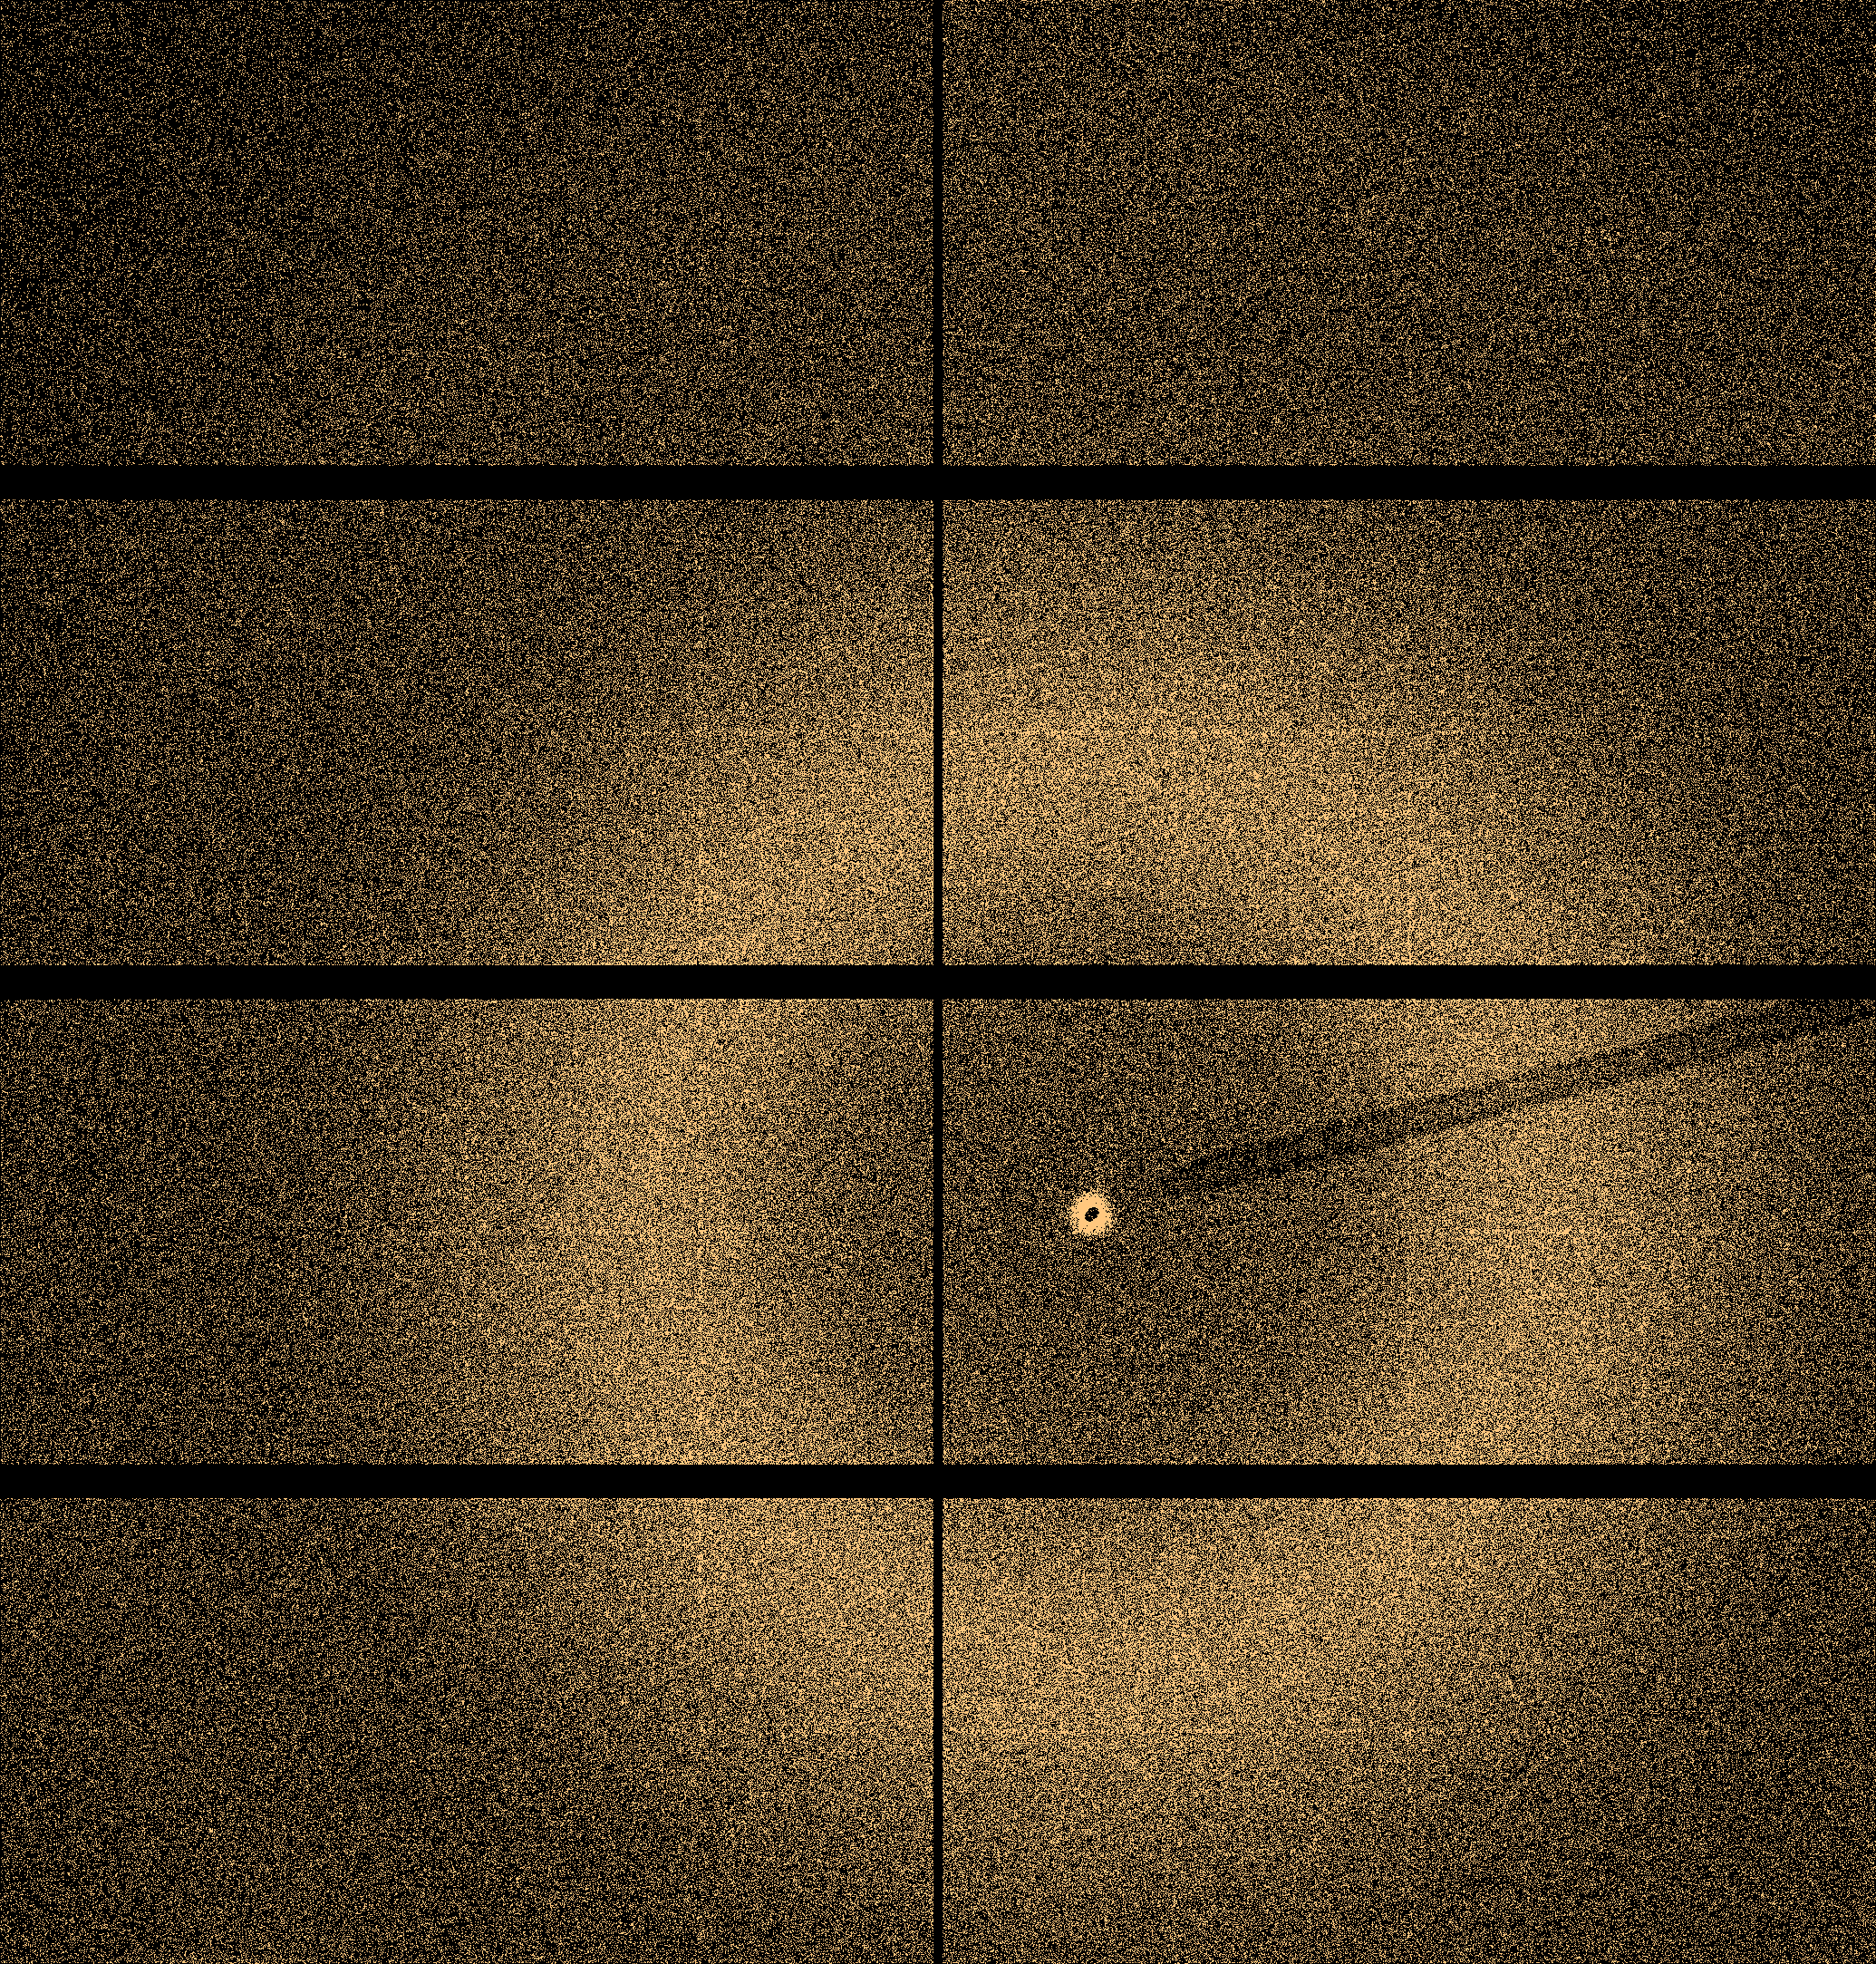
\includegraphics[width=0.9\linewidth]{fig/obj.png}
    \vspace{3px}
    \caption{Изображение с 2D~-детектора. Черные области соответствуют промежуткам между элементами детектора, затемненная облась справа  - тень от заслонки}
    \label{fig:difractogram}
%  \end{center}
\end{wrapfigure}
	
	
	Детектирование картин дифракции при сканировании образца наноразмерным пучком рентгеновского синхротронного излучения производится с шагом 1 мкм. 
	Это позволяет установить, что изучаемые порошки и пленки не являются однородными, а имеют как чисто аморфные, так и частично-кристаллические участки.
	Типичное изображение, получаемое на детекторе для единичного измерения, представлено на рис. \ref{fig:difractogram}. 
	
	\begin{figure}[t]\center
\begin{tabular}{cc}
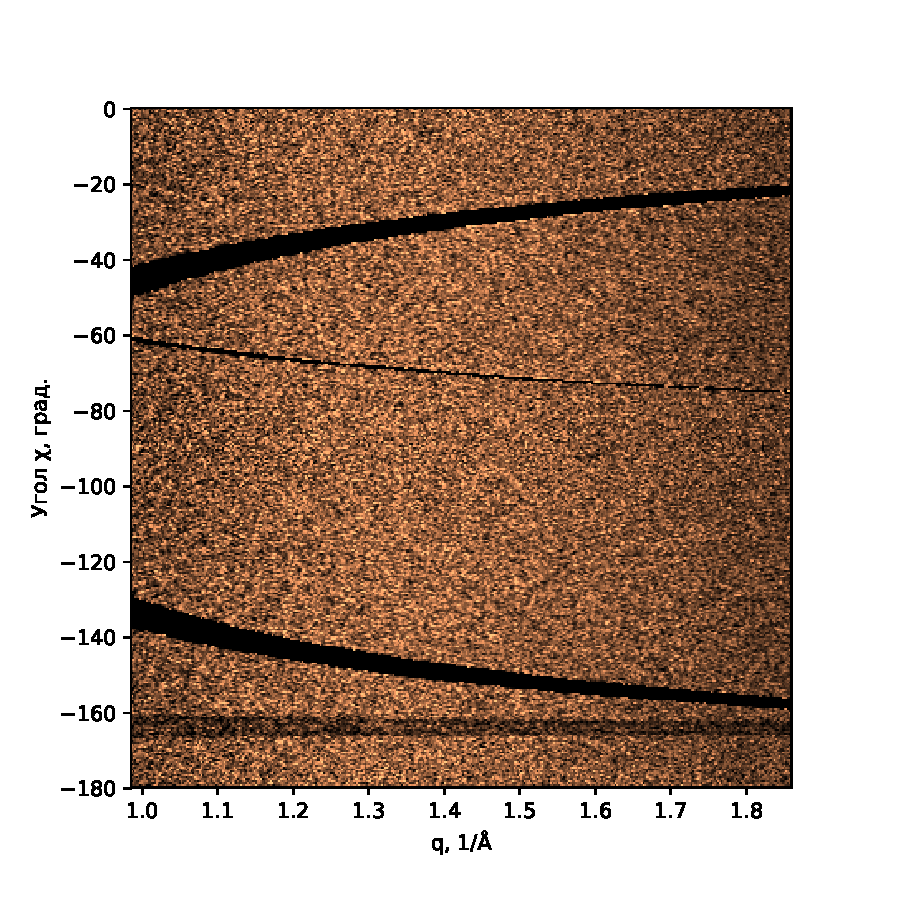
\includegraphics[width=0.5\linewidth]{fig/azim-amo.pdf}
&
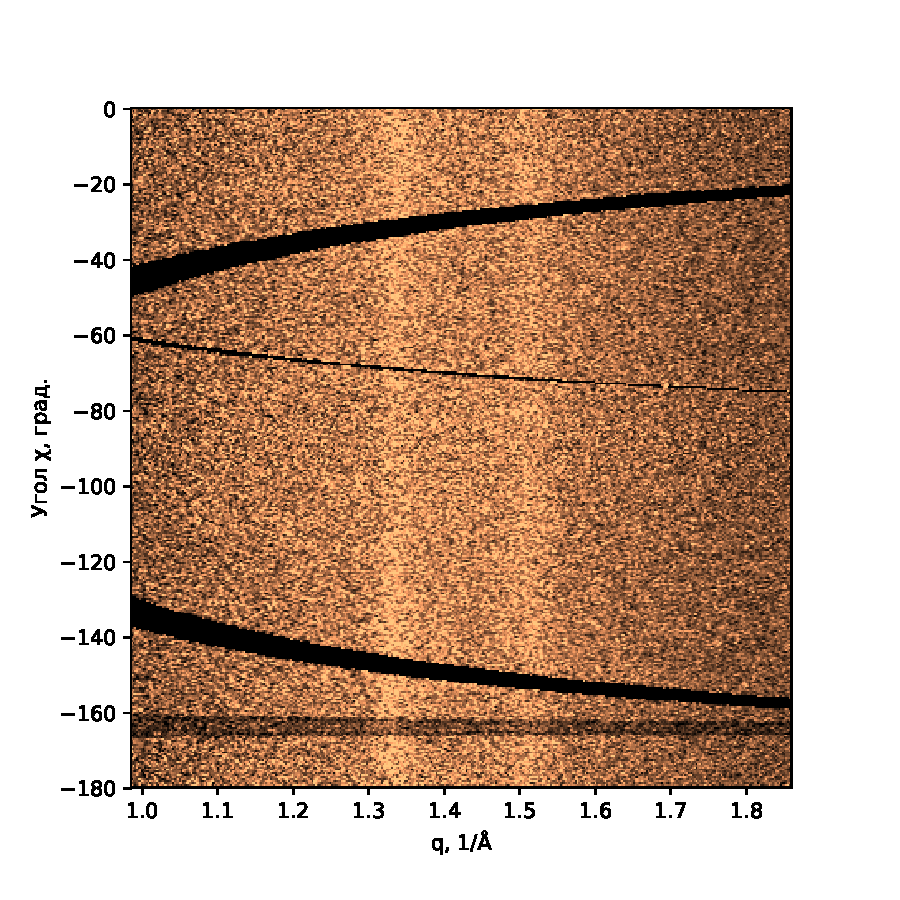
\includegraphics[width=0.5\linewidth]{fig/azim-cryst.pdf}
\end{tabular}
\caption{Фрагменты дифрактограмм (в координатах $(q,\chi)$) в аморфной (слева) и кристаллической (справа) областях.}
\label{fig:azim}
\end{figure}

	

	
	Различие в сигналах кристаллических и аморфных областей хорошо видно на фрагментах дифрактограмм, преобразованных к полярной системе координат, представленных на рис. \ref{fig:azim}. 
	Как видно из рисунка, наличие кристаллической фазы приводит к появлению  дифракционных пиков, в то время как рассеяние на чисто аморфных участках дает только так называемое аморфное гало.
	
В результате азимутального интегрирования получаются одномерные профили дифракции, как, например, профиль на рис.  \ref{fig:waxs_profile}.

		\begin{figure}[h]
    \centering
    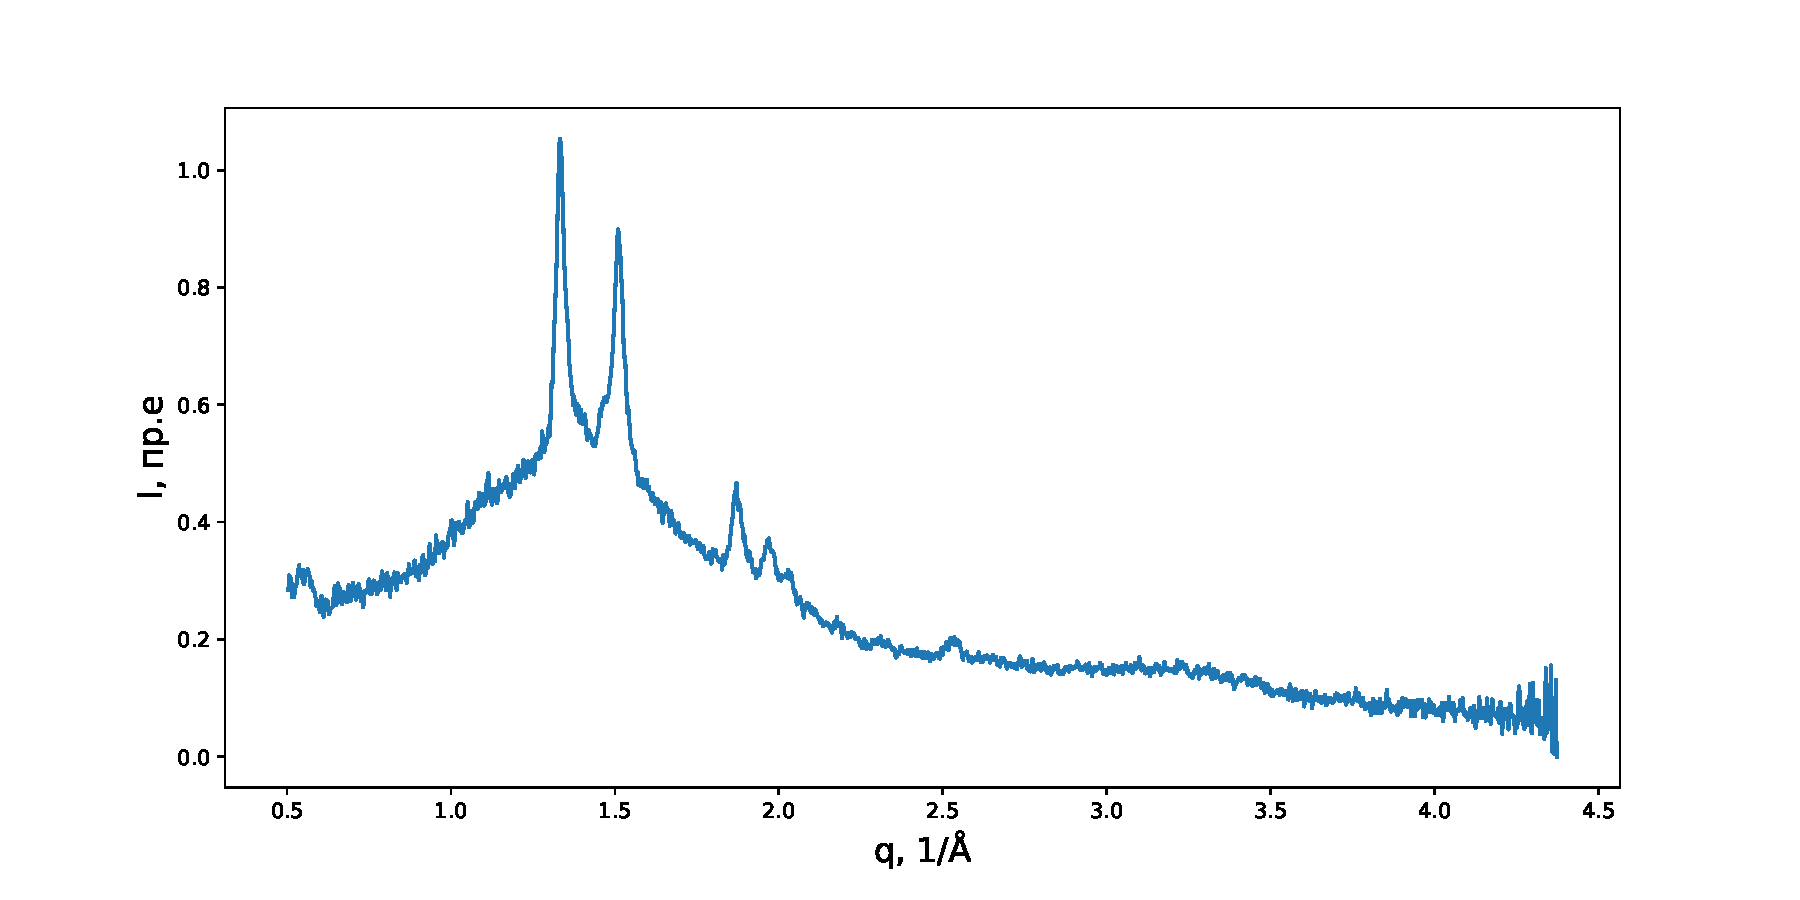
\includegraphics[width=\linewidth]{fig/profile.pdf}
    \caption{Картина дифракции в частично-кристаллической области после азимутального интегрирования}
    \label{fig:waxs_profile}
\end{figure}
	

\subsection{Вычитание фона}

	
			\begin{wrapfigure}[4]{l}{0.4\linewidth}
\singlespacing
\vspace{-35px}
%  \begin{center}
    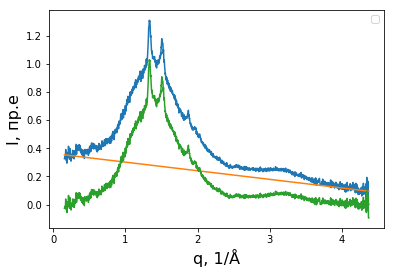
\includegraphics[width=\linewidth]{fig/base.png}
    \vspace{3px}
    \caption{Вычитание фона}
    \label{fig:base}
%  \end{center}
\end{wrapfigure}


Фоновый сигнал, не относящийся к рассеянию на изучаемом образце, приближенно аппроксимируется прямой, как показано на рис. \ref{fig:base}.



\section{Распознавание сигнала аморфной фазы}

	
	Для расчета индекса кристалличности при обработке данных дифракции необходимо распознание кристаллических пиков и сигнала от аморфной фазы.
	В отличие от обычного фона, широкие пики рассеяния от аморфной фазы нельзя определить один раз для всех измерений, так как его форма зависит от степени кристалличности. Таким образом, его оценку необходимо проводить для каждого профиля отдельно.
	Стандартные алгоритмы для автоматического распознавания фона, основанные на полиномиальной аппроксимации, показали себя неэффективными в нашем случае. Распознавание кристаллических пиков и аморфного фона производилось с помощью фильтра "rolling ball". В рентгеноструктурном анализе он как правило применяется к двумерным дифрактограммам кристаллических материалов, как например, в работе \cite{ball2018}. Однако подходящая реализация для одномерных профилей, не представлена в открытых источниках. Ниже (листинг \ref{lst:ball}) приведена реализация алгоритма для одномерных профилей на языке Python, которая применяется далее для определения кристалличности исследуемых образцов. Остальныя процедуры обработки данных также производилось с помощью Python и представлены в \cite{git}.
	 
\vspace{5px}
	\begin{lstlisting}[language=Python, caption= Реализация распознавание кристаллических пиков по алгоритму "rolling ball", label={lst:ball}]
import numpy as np

def rolling_ball(profile, r):
    #r - ball radius
    #profile - 1D profile, smoothed
    t1 = np.full(profile.shape[0], np.amax(profile), dtype=np.float32)
    for i in range (t1.shape[0]):
        for j in range(-r,r):
            if ((i+j)>0 and (i+j)<t1.shape[0]):
                if(t1[i]>profile[i+j]):
                    t1[i]=profile[i+j]
                    
    t2 = np.zeros(profile.shape[0],dtype=np.float32)
    count = np.zeros(profile.shape[0],dtype=np.float32)
    back = np.zeros(profile.shape[0],dtype=np.float32) 
    
    for i in range(t2.shape[0]): 
        for j in range(-r,r):
            if ((i+j)>0 and (i+j)<t2.shape[0]):
                t2[i]+=t1[i+j]
                count[i]+=1
        back[i] = t2[i]/count[i]
    return back
 

\end{lstlisting}
\vspace{5px}

	Принцип действия алгоритма проиллюстрирован на рис. \ref{fig:ball}. 
	Его можно представить как круг заданного радиуса, который "катится"  под графиком \cite{ball2018}.Траектория его центра образует линию, которая и вычитается из начального профиля. 
		\begin{figure}[ht]
	    \centering
	    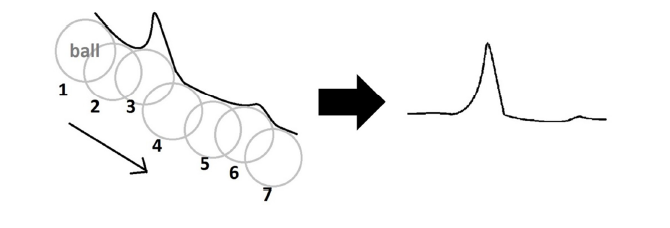
\includegraphics[width=\linewidth]{fig/ball.PNG}
	    \caption{Процедура вычитания фона.}
	    \label{fig:ball}
	\end{figure}

	
	Пики, чья ширина меньше радиуса круга, не вычитаются, и остаются в конечном профиле. Так, алгоритм позволяет убирать широкий сигнал рассеяния  на аморфной фазе, и оставлять только узкие кристаллические пики (рис. \ref{fig:ball-profile}).
	
	
	\begin{figure}[ht]
	    \centering
	    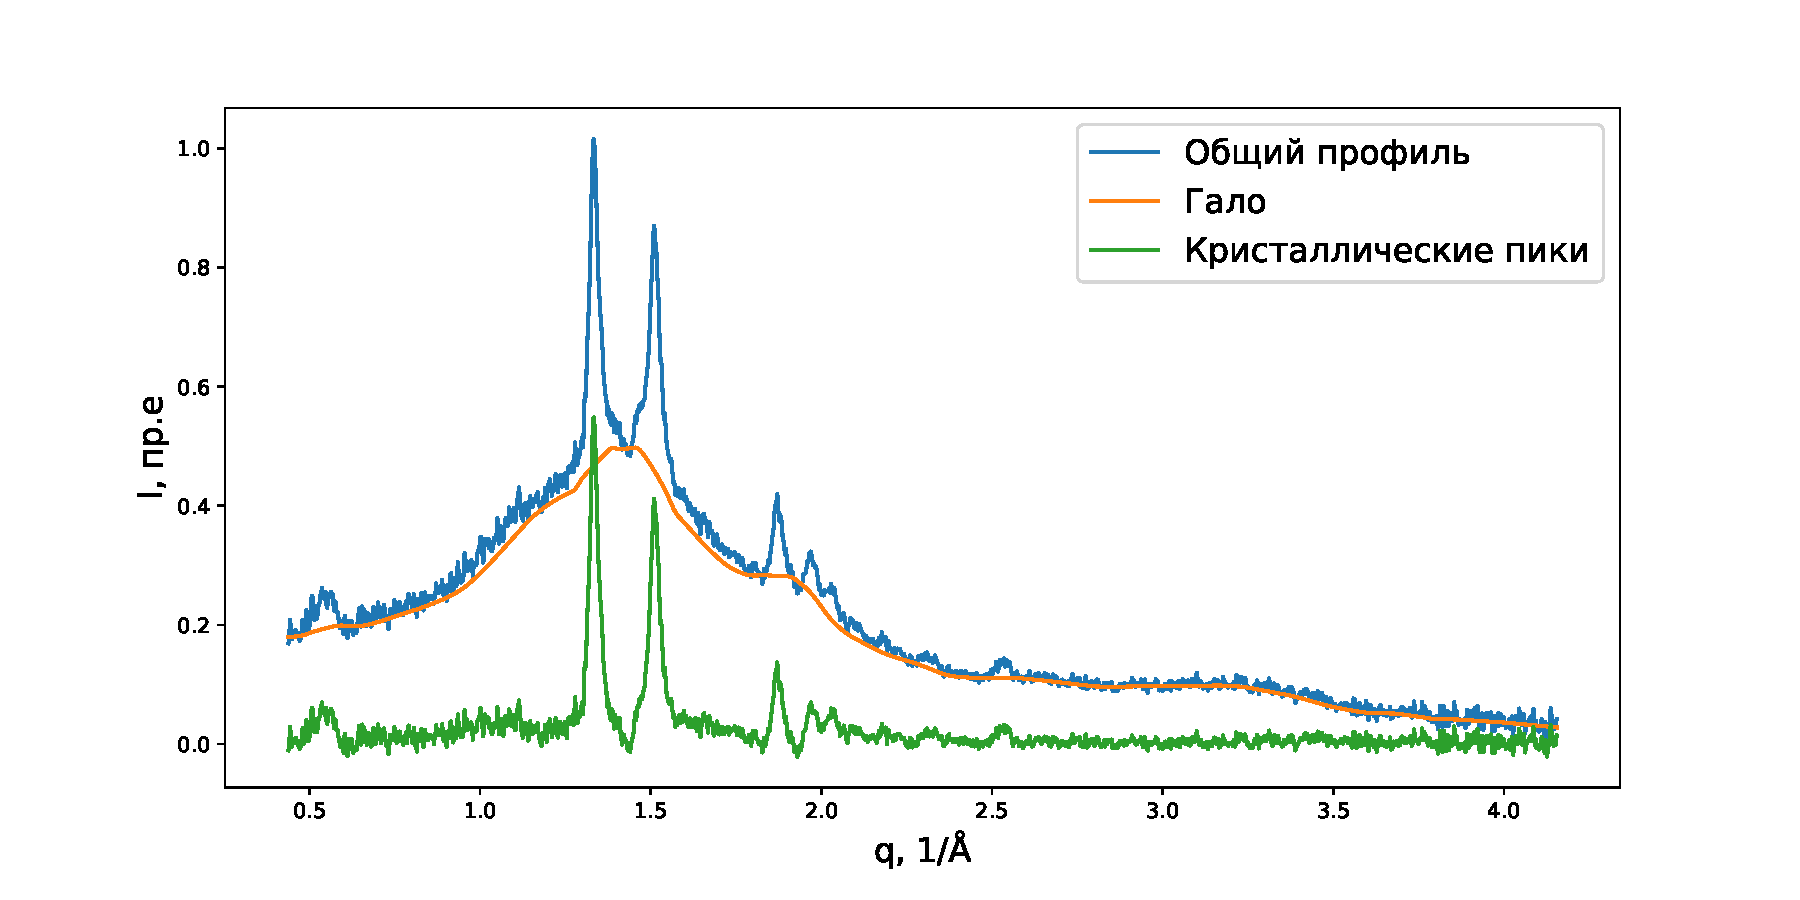
\includegraphics[width=\linewidth]{fig/ball-profile.pdf}
	    \caption{Распознавание аморфного гало}
	    \label{fig:ball-profile}
	\end{figure}



\section{Картография образцов}

\subsection{Порошки}

По данным оптической микроскопии, размеры частиц порошка составляют $5.8\pm 2.8$ мкм,и имеют мономодальное распределение. Составление карт кристалличности образцов показывает, что сами порошки состоят из частичнокристаллических частиц заявленных размеров, с индексом кристалличности около 0.1. На рис.\ref{fig:powder} показана микрограмма частиц порошка, а также карты кристалличности для исследуемых порошковых образцов.


	\begin{figure}[h]
	    \centering
	    \begin{tabular}{ccc}
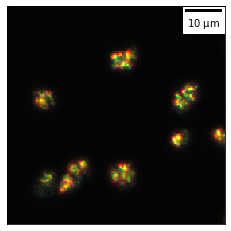
\includegraphics[width=0.26\linewidth]{fig/powder_optic.png}
&
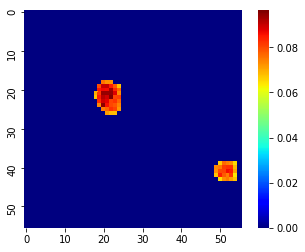
\includegraphics[width=0.33\linewidth]{fig/1416map.png}
&
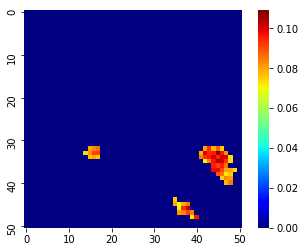
\includegraphics[width=0.33\linewidth]{fig/1434map.png}
\end{tabular}
	    \caption{Отдельные частицы}
	    \label{fig:powder}
	\end{figure}
	
Графики на рис. \ref{fig:var-profile} показывают, как изменяется интенсивность кристаллических пиков в различных областях карты: месте отсутсвия образца, не периферии и в центре частицы.

\begin{figure}[h]
    \centering
    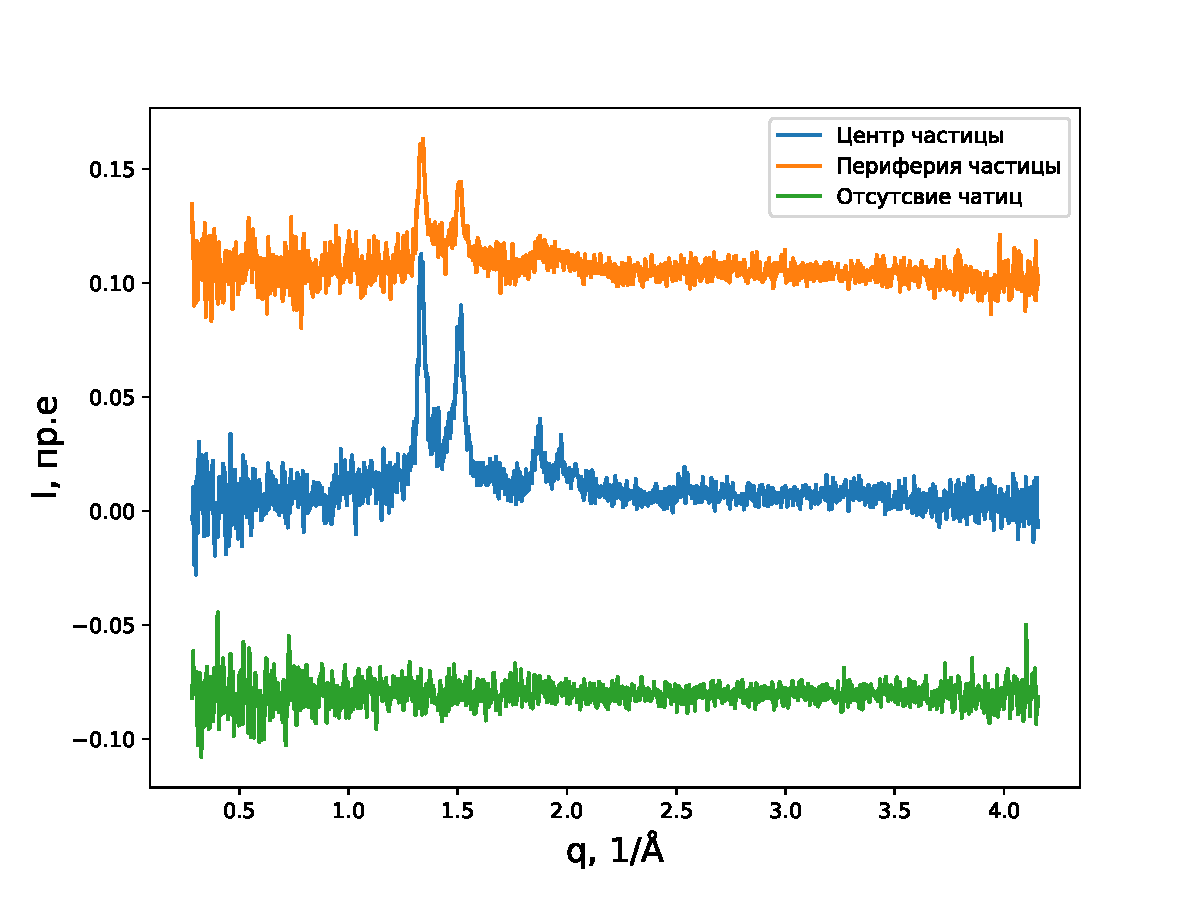
\includegraphics[width = \linewidth]{fig/var-profile.pdf}
    \caption{Сигнал кристаллической фазы в разичных областях карты кристалличности частиц порошка}
    \label{fig:var-profile}
\end{figure}

	
		\begin{figure}[h]\centering
\begin{tabular}{cc}
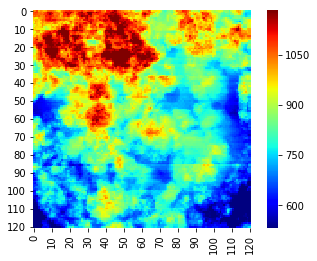
\includegraphics[width=0.5\linewidth]{fig/example72.png}
&
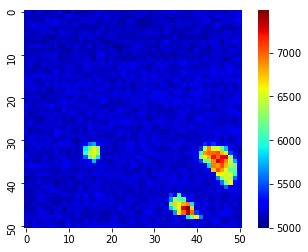
\includegraphics[width=0.5\linewidth]{fig/example1434.png} \\
\end{tabular}
\caption{Карты кристалличности}
\label{fig:maps_powder}
\end{figure}
	
	
	
%\section{Расчет характеристик}
